\section{美国流感住院数据的检验}
\label{sec:empirical}

本节用美国流感住院周报检验误差是否呈“常数加规模反比”的形状，分析拟合的截距与斜率为何高于理论值，并考察疫情阶段和报告制度变化时这一形状的变化。

\subsection{数据与口径}
\label{sec:empirical-data}

数据来自美国国家医疗安全网络（NHSN）公布的各辖区每周实验室确诊流感住院数，以及各辖区填报医院所占比例\citep{cdc2026nhsn}。样本覆盖 50 个州与华盛顿特区，共 16,218 个州周。其中 504 个州周的住院数缺失，按 0 处理，其中 468 个在第一期，36 个在第二期。

规模用此前三周报告数的加权和度量
\begin{equation}
  D_t=0.65\,C_t+0.25\,C_{t-1}+0.10\,C_{t-2}.
  \label{eq:dt}
\end{equation}
相对待预测的 $C_{t+1}$，$D_t$ 的平均回溯滞后为 1.45 周，约 10.2 天。增长统计量取 $G_t=C_{t+1}/D_t$。只保留 $D_t\geq5$ 的州周，得到 10,303 个有效观测。

$G_t$ 与第~\ref{sec:model}~节的 $R_t$ 不是同一个量。流感的世代间隔约 3 天，一周约跨两代，$G_t$ 是两代左右增长的合成，其均值和方差都不等于单代再生数的均值和方差。所以下文只用模型的结构，即误差随规模的形状，不把拟合得到的系数解读为单代参数的估计。

误差指标采用相对均方误差。以某一阶段的平均增长比 $\Rbar$ 为基准，第 $t$ 周的损失为 $L_t=[(G_t-\Rbar)/\Rbar]^2$。由式~\eqref{eq:identity}，它也是用 $\Rbar D_t$ 预测 $C_{t+1}$ 的相对误差平方，属于常用的相对误差评分\citep{bosse2023scoring}。在单代模型下，以预计报告规模 $m$ 代替 $D_t$，有
\begin{equation}
  \E(L_t\mid D_t)\approx a+\frac{b}{D_t},\qquad a=\frac{v_R}{\Rbar^2},\quad b=\frac{A}{\Rbar^2},\quad \frac ba=\mx.
  \label{eq:affine}
\end{equation}
式~\eqref{eq:affine} 是下文的拟合形式。$b/a$ 称为经验交叉点。

样本期内 NHSN 的填报制度变过两次（图~\ref{fig:nhsn}）。2020 年 10 月至 2024 年 4 月 30 日为强制填报，下称第一期，有效观测 6,009 个，平均填报率 91.1\%。2024 年 5 月 1 日至 10 月 31 日改为自愿填报，下称第二期，有效观测 420 个，平均填报率 54.6\%，中位数 45.7\%。2024 年 11 月 1 日起，美国联邦医疗保险与医疗补助服务中心恢复强制要求，下称第三期，有效观测 3,874 个，平均填报率 91.8\%。

\begin{figure}[!tbp]
  \centering
  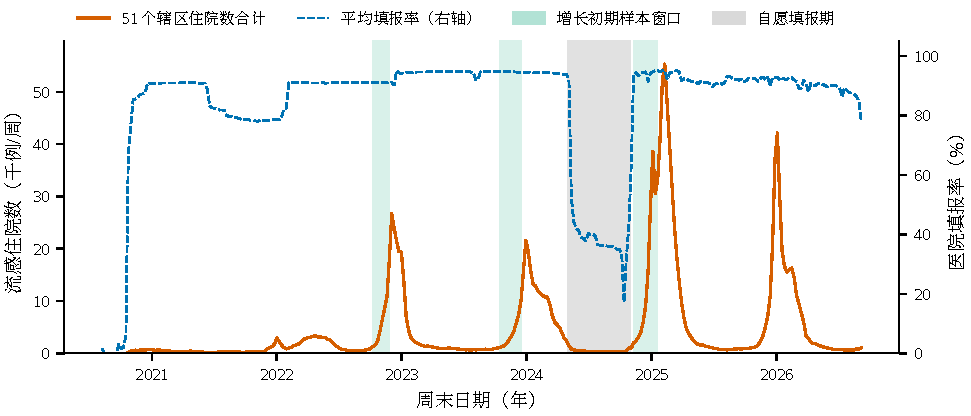
\includegraphics[width=\textwidth]{figures/fig_05_fig05_nhsn_series.pdf}
  \caption{美国 51 个辖区每周流感住院数合计（实线，左轴）与医院平均填报率（虚线，右轴）。缺失按 0 计入合计。绿色区间为三个流行季的增长初期样本窗口，灰色区间为 2024 年 5--10 月的自愿填报期。}
  \label{fig:nhsn}
\end{figure}

\subsection{流行初期的规模效应}
\label{sec:empirical-early}

模型假定各期环境围绕同一均值波动。流行初期最接近这一情形，所以主分析取三个流行季的增长初期，即 2022 年 10 月 8 日至 11 月 26 日，2023 年 10 月 14 日至 12 月 16 日，2024 年 11 月 9 日至 2025 年 1 月 18 日。窗口内共 1,267 个有效州周，平均增长比 $\Rbar_{\mathrm{early}}=1.6706$，标准差 0.7116。

误差随规模下降，并逐渐趋平（图~\ref{fig:early}）。按 $D_t$ 分为六箱，$[5,20)$ 箱的平均损失为 0.329（$N=319$，95\% 区间 0.244--0.415），$[20,50)$ 箱降到 0.161，$[100,250)$ 箱为 0.112，此后两箱停在 0.103 和 0.105 附近。

\begin{figure}[!tbp]
  \centering
  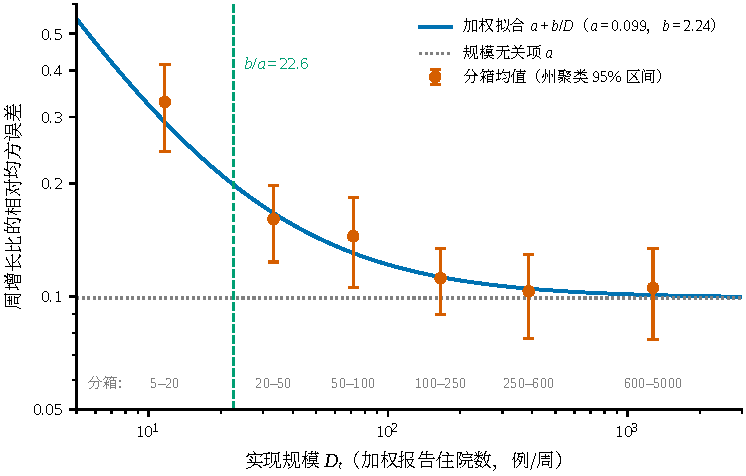
\includegraphics[width=0.8\textwidth]{figures/fig_06_fig06_early_scale.pdf}
  \caption{流行初期单步预测误差随实现规模 $D_t$ 的变化，共 1,267 个州周。圆点为各分箱均值，画在箱内平均 $D_t$ 处，误差棒为按州聚类重抽的 95\% 区间；曲线为 $a+b/D$ 的拟合，水平虚线为截距 $a$，竖线为经验交叉点 $b/a$。}
  \label{fig:early}
\end{figure}

我们用可行广义最小二乘拟合式~\eqref{eq:affine}，权重取 $1/\hat\mu^2$，$\hat\mu$ 为一步拟合值\citep{wooldridge2010econometric}；区间由按州聚类的 1,500 次重抽给出\citep{cameron2008bootstrap, cameron2015practitioner}。结果为 $a=0.0991$（95\% 区间 0.0841--0.1173），$b=2.2434$（1.5019--3.0161），1,500 次重抽中没有一次 $b\leq0$。经验交叉点 $b/a=22.6$ 例/周（13.7--33.7）。用十分位分组均值拟合，交叉点同样为 22.6。

权重的选择只影响效率，不影响一致性。损失的离散程度随规模收缩，$\Var(L)/\E(L)^2$ 从最小箱的 5.32 降到最大箱的 0.99，所以 $1/\hat\mu^2$ 并非最优权重。不过权重只依赖 $D_t$，拟合仍然一致；普通最小二乘给出 $b=2.305$，与 2.243 接近。

交叉点对极端值敏感。去掉损失最大的 1\% 观测后，$a=0.1077$，$b=1.137$（0.697--1.661），交叉点降到 10.6（5.9--17.3）。两项单向聚类的敏感性分析结论不变。每次重抽都重新估计基准 $\Rbar_{\mathrm{early}}$，$b$ 的 95\% 区间为 1.517--2.981；改为按周聚类，区间为 1.473--3.119。州与周两个维度的双向聚类没有做，原因见第~\ref{sec:discussion}~节。

把平均损失拆开，可以看出扩大规模还剩多少空间。样本平均损失为 0.181，截距 $a$ 占 54.6\%，规模项 $b/D_t$ 占 45.1\%，拟合残差占 0.2\%；规模项按 $D_t$ 的调和平均数 27.4 计算。若所有州周的规模都提高到 250，模型给出的平均损失为 0.107，下降 40.9\%。实际 $D_t\geq250$ 的 244 个州周平均损失为 0.104，约为全样本均值的六成。后一个数与模型上限 0.108 接近，但它由拟合机械地决定，不构成独立证据。

经验交叉点 22.6 与理论情景区间同一量级。情景参数取 $\Rbar=1.67$，$k\in[0.2,0.5]$\citep{lloydsmith2005superspreading}，$\rho\in[0.0056,0.021]$\citep{zhou2012hospitalizations, tokars2018seasonal}，$v_R\in[0.04,0.08]$，此时 $A$ 在 1.702--1.967，$\mx$ 在 21.3--49.2。但比值吻合不能当作对结构参数的检验。情景隐含的截距为 0.0143--0.0287，斜率为 0.610--0.705；实证 $a$ 是前者的 3.5--6.9 倍，$b$ 是后者的 3.2--3.7 倍。两者被放大的倍数相近，比值才碰巧落在区间内。

\subsection{截距与斜率为什么偏大}
\label{sec:empirical-inflation}

偏大有两个来源，分别作用于斜率和截距。

分母噪声主要抬高斜率。$D_t$ 本身是带二项报告噪声的计数，比真实感染压力 $\rho\Lambda_{t+1}$ 多一层随机性。用 delta 方法展开，斜率近似为
\begin{equation}
  b\approx\frac{A+(1-\rho)(\Rbar^2+v_R)\sum_s {w_s}^2}{\Rbar^2},
  \label{eq:b-delta}
\end{equation}
其中 $\sum_s {w_s}^2$ 是式~\eqref{eq:dt} 中滞后权重的平方和。权重越集中，$D_t$ 越接近单周计数，噪声越大，$b$ 也越大。这与测量误差文献中分母或自变量含噪时的系数偏移是同一类问题\citep{fuller1987measurement, carroll2006measurement}。

式~\eqref{eq:b-delta} 预测的是不同滞后权重之间 $b$ 的相对变化，这一点与数据吻合（图~\ref{fig:noise}a）。我们比较三种权重，即主规格（0.65/0.25/0.10，$\sum w^2=0.495$）、只用当周（$\sum w^2=1$）和三周等权（$\sum w^2=0.333$）。实证斜率依次为 2.243、3.134（2.203--4.067）和 1.926（1.071--2.807）。相对主规格，后两者的比值为 1.40 和 0.86；式~\eqref{eq:b-delta} 在情景参数下的预测为 1.44 和 0.86。情景参数取 $\Rbar=1.67$，$v_R=0.06$，$k=0.35$，$\rho=0.021$，$A=1.8409$。预测斜率为 1.155、1.660、0.993，模拟值为 1.195、1.566、0.999。

水平上，分母噪声只解释了一部分。没有分母噪声时，情景斜率为 0.660，约为实证值的 29\%；加入二项噪声后升到 1.155，约为 51\%。剩余部分的一个可能来源是报告过程的超额离散，把报告离散度设为 $\varphi=1.96$ 时，模拟斜率为 2.019。这只是可能的解释之一，数据本身无法区分。

分母噪声只抬高斜率，不抬高截距。情景模拟中三种权重的截距为 0.0225、0.0202、0.0214，几乎不变，于是 $b/a$ 被推高到 59.2，而真实的 $A/v_R$ 只有 30.7。因此，用 $b/a$ 估计 $\mx$ 会系统性偏大。

截距的放大另有来源。实证截距随回溯滞后单调上升，平均滞后为 1.0、1.45、2.0 周时，$a$ 分别为 0.0682、0.0991、0.1524（图~\ref{fig:noise}b），都远高于情景隐含的 0.014--0.029；模拟中截距不随滞后变化。这与式~\eqref{eq:mse-decomp} 的条件偏差项一致。真实的 $R_t$ 有时间相关，分母越陈旧，$\mu_t/D_t$ 偏离 $\Rbar$ 越远，偏差项越大。前面提到的 $G_t$ 跨两代左右，也会放大与规模无关的波动。

\begin{figure}[!tbp]
  \centering
  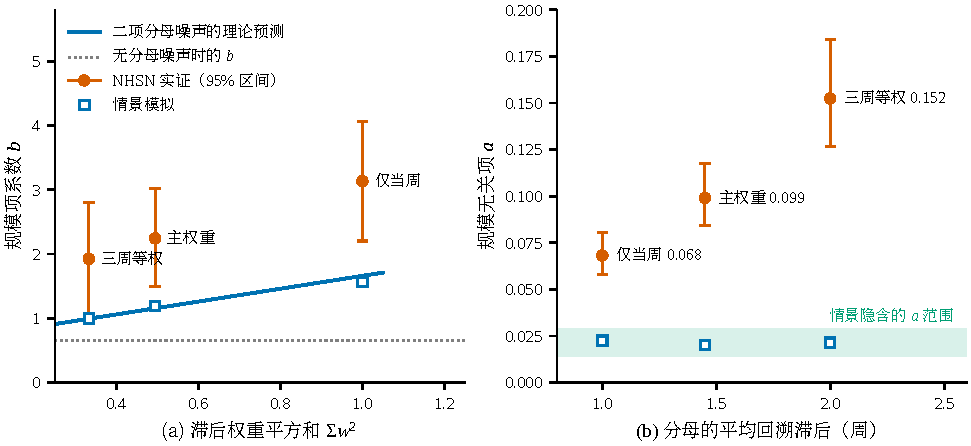
\includegraphics[width=\textwidth]{figures/fig_07_fig10_denominator_noise.pdf}
  \caption{滞后权重对拟合系数的影响。(a) 规模项系数 $b$ 与滞后权重平方和 $\sum w^2$ 的关系：圆点为三种权重的实证估计及 95\% 区间，方块为情景模拟值，斜线为二项分母噪声的一阶近似，水平虚线为没有分母噪声时的 $b$。(b) 截距 $a$ 与分母平均回溯滞后的关系，阴影为情景隐含的截距范围 0.014--0.029。}
  \label{fig:noise}
\end{figure}

在三种滞后权重下，规模项都为正，误差形状稳定。经验交叉点则随权重在 12.6--46.0 之间变化，它描述 $G_t$ 这一统计量的误差结构，不能当作 $A/v_R$ 的估计。

\subsection{达峰期与报告制度变化}
\label{sec:empirical-peak}

流行达峰后，基准本身失效。取三个流行季的全国峰值周（2022 年 12 月 3 日、2023 年 12 月 30 日、2025 年 2 月 8 日）及其后 7 周，共 1,220 个州周，平均增长比降到 $\Rbar_{\mathrm{peak}}=0.8075$，标准差 0.3048。若继续用初期均值 1.6706 作基准，各箱的平均损失都在 0.29--0.31，看不出随规模下降。

图~\ref{fig:peak} 把这部分损失拆成两块，即基准偏移造成的常数偏差 $(\Rbar_{\mathrm{early}}-\Rbar_{\mathrm{peak}})^2/\Rbar_{\mathrm{early}}^2=0.2669$，以及箱内围绕峰期均值的波动。偏差项占总损失的 88.9\%，从最小箱的 59.5\% 升到最大箱的 94.8\%。除最小箱外，峰期损失是同箱初期损失的 1.8--2.9 倍。

\begin{figure}[!tbp]
  \centering
  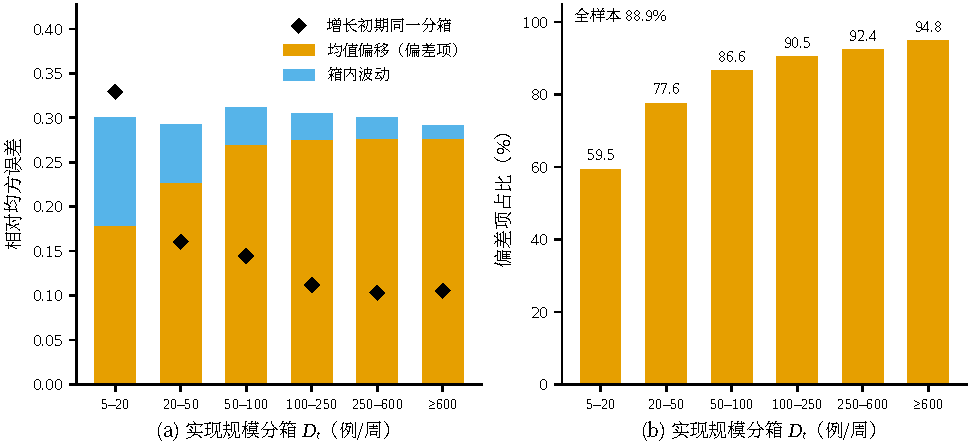
\includegraphics[width=\textwidth]{figures/fig_08_fig07_peak_decomp.pdf}
  \caption{达峰期（峰值周及其后 7 周）以流行初期均值为基准时的误差分解。(a) 各规模箱的平均损失，分为基准偏移造成的偏差项与箱内波动，菱形为同一分箱在流行初期的平均损失。(b) 偏差项在各箱损失中的占比。}
  \label{fig:peak}
\end{figure}

改用峰期自身均值作基准后，规模效应重新出现，$a=0.0665$（0.0467--0.0897），$b=7.927$（5.424--11.225），交叉点 119.2（64.0--225.9），平均损失 0.142。这里的 $b$ 不能直接和初期的 2.243 比较，因为两者的归一化分母不同。统一用 $\Rbar_{\mathrm{early}}$ 归一化后，峰期斜率为 1.852，低于初期的 2.243；不归一化时为 5.169 对 6.261。同一样本上的联合回归中，阶段交互项为 $-0.92$，95\% 区间 $-2.33$--$0.59$，包含零。所以达峰期规模仍然有用，但没有证据表明它比初期更有用或更没用。达峰期应当换用能跟踪基准变化的模型，同时继续维持病例规模。

报告制度变化提供了另一类证据（图~\ref{fig:policy}）。从第一期到第二期，$G_t$ 的标准差从 0.624 升到 1.823，增加 192\%；第三期回到 0.649。稳健离散度几乎不动。四分位距为 0.638、0.594、0.652，第二期反而略低；中位绝对偏差为 0.298、0.299、0.292。偏度从 3.29 升到 14.98，再回到 2.68；$G_t$ 的最大值从 12.7 升到 33.9。

\begin{figure}[!tbp]
  \centering
  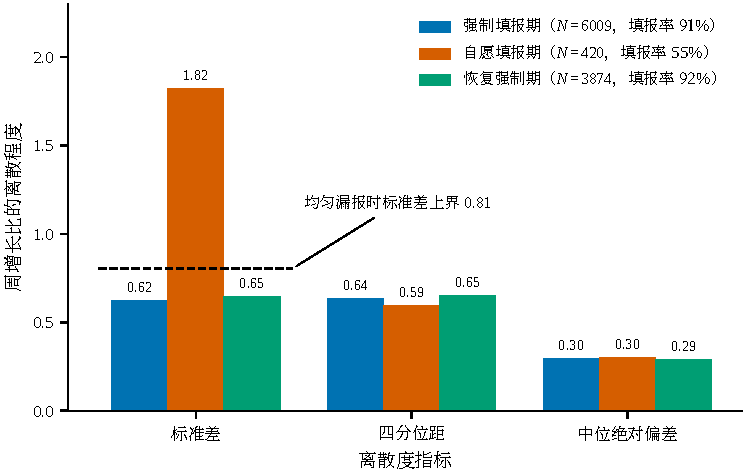
\includegraphics[width=0.8\textwidth]{figures/fig_09_fig08_reporting_policy.pdf}
  \caption{三个填报制度期内周增长比 $G_t$ 的离散程度。柱上数字为指标值。虚线为填报率从 91.1\% 降至 54.6\% 时，若漏报在医院间均匀发生，第二期标准差可能达到的上限。}
  \label{fig:policy}
\end{figure}

若填报率下降只是均匀地稀疏了病例，标准差最多放大到 $0.624\times\sqrt{91.11/54.59}=0.806$，即 1.29 倍。实际放大了 2.92 倍，而且只有标准差放大、分位数指标不变。这说明扩张来自少数极端周，例如部分医院时报时不报造成的跳变；整体噪声并没有均匀增加。它与命题~\ref{prop:reporting} 只有定性联系。报告率下降会增加方差，但第二期的主要变化是结构性扰动，无法用 $\rho$ 的变化定量解释。

\subsection{稳健性与外部对照}
\label{sec:empirical-robust}

图~\ref{fig:forest} 汇总了各规格下的经验交叉点。规模项在所有规格下都为正；交叉点在 10.6--124.7 之间变化，这说明它只能作量级参考。

\begin{figure}[!tbp]
  \centering
  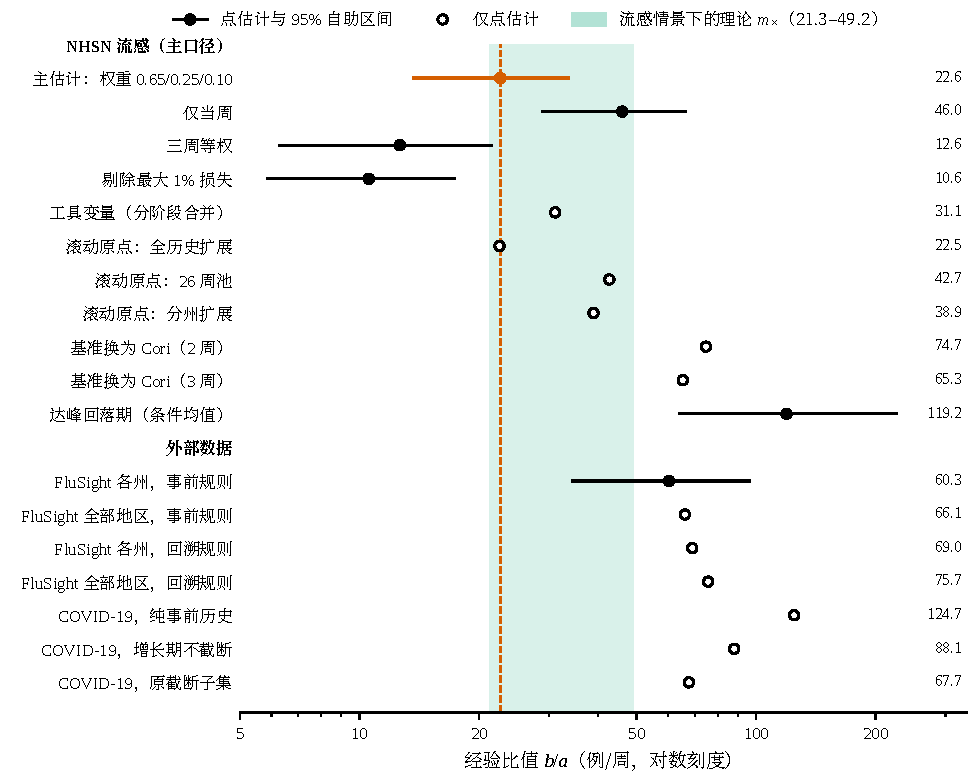
\includegraphics[width=\textwidth]{figures/fig_10_fig09_mx_forest.pdf}
  \caption{各规格下的经验交叉点 $b/a$。横线为 95\% 区间（只有部分规格提供），阴影为理论情景区间 21.3--49.2，竖直虚线为主估计 22.6，右侧列出点估计。上部为 NHSN 数据的不同规格，下部为外部数据。}
  \label{fig:forest}
\end{figure}

\subsubsection{替代性滞后测度}

$D_t$ 与 $C_{t+1}$ 同源，同期测度可能带来内生性。用滞后 3--5 周的规模作 $1/D_t$ 的工具变量，在流行季内合并样本（$N=1{,}051$）上做两阶段最小二乘\citep{wooldridge2010econometric}，得到 $b_{\mathrm{iv}}=2.53$（1.11--4.11），同一样本的普通最小二乘为 1.35，两者之差的 95\% 区间为 0.30--2.11；对应交叉点 31.1。第一阶段 $F$ 统计量为 1147.1，按州聚类为 312.9。排除限制无法检验，所以工具变量估计只说明在替代性滞后测度下，规模项保持为正。$b_{\mathrm{iv}}$ 高于普通最小二乘，与测量误差造成的衰减偏误方向一致\citep{fuller1987measurement}。

\subsubsection{事前基准}

主分析的基准 $\Rbar_{\mathrm{early}}$ 用到了整个窗口的数据，属于回顾性口径。改用只含过去信息的基准后，误差整体上升。全部历史扩张窗的 $a=0.406$，$b=9.158$（5.82--12.88）；26 周滚动池的 $a=0.222$，$b=9.456$；逐州扩张窗的 $a=0.341$，$b=13.27$。三种口径下所有重抽的 $b$ 都为正，交叉点在 22.5--42.7。截距在总损失中的份额随口径在 39\%--55\% 移动。

\subsubsection{时变基准}

用 \citet{cori2013new} 的滑动窗口估计 $R_t$ 作预测，2 周窗与 3 周窗的平均损失为 0.288 和 0.249，阶段均值基准为 0.181，直接用本周病例数预测下周的朴素方法为 0.637。对 Cori 基准的损失拟合式~\eqref{eq:affine}，2 周窗 $a=0.0812$、$b=6.064$，交叉点 74.7；3 周窗交叉点 65.3。时变估计在小规模时自身噪声大，所以斜率更陡。

\subsubsection{空间汇总}

全国加总序列的流行初期平均规模约 6,662 例/周，平均损失降到 0.0348（中位数 0.0115，$N=28$），约为单州截距的三分之一。按式~\eqref{eq:pooling}，这对应一个小于 1 的州间环境相关 $\bar c$，粗略推算约为 0.34。这一推算忽略了分母噪声和 $G_t$ 的口径问题，只能当作量级。

\subsubsection{外部数据}

FluSight 是美国疾病控制与预防中心组织的流感住院前瞻预测，我们使用其 2022--2023 季的集成预测\citep{mathis2024evaluation}，相关评价框架见文献\citep{reich2019accuracy, cramer2022evaluation}。以集成模型事前给出的预测规模 $\widehat Y\geq5$ 筛选州级样本（$N=1{,}177$），$a=0.1295$，$b=7.805$（5.358--10.526），交叉点 60.3（34.5--95.9）；其余三种筛选口径为 66.1、69.0 和 75.7。把该集成预测在各流行阶段内的相对均方误差拆成均值偏差平方与阶段内方差两部分，均值偏差平方在峰期（$N=206$）占 15.5\%，在上升期（$N=216$）和回落期（$N=755$）分别占 32.3\% 和 1.5\%。欧洲 11 国 2020 年 2--4 月的 COVID-19 序列\citep{flaxman2020estimating} 给出更大的交叉点。纯事前口径 $N=404$，$b=33.92$（14.60--74.99），交叉点 124.7；只取增长期为 88.1，截断子样本为 67.7。两组外部数据中规模项都为正，交叉点高于 NHSN 主估计。病种、预测方法和报告系统都不同，这些数字不宜直接比较大小。
